%%%%%%%%%%%%%%%%%%%%%%%%%%%%%%%%%%%%%%%%%%%%%%%%%%%%%%%%%%%%%%%%%%%%%%%%%%%%%%%%%%%%

\section{Recursão}

%%%%%%%%%%%%%%%%%%%%%%%%%%
\begin{frame}
\frametitle{Recursão}
\begin{minipage}{0.47\textwidth}
    \begin{itemize}
        \item Contextualizar a recursão
        \item Princípios
        \item 03 exemplos
        \item \textit{Backtracking}
    \end{itemize}
\end{minipage}
\begin{minipage}{0.5\textwidth}
\begin{figure}[ht!]
\begin{center}

\includegraphics[width=1.2\textwidth, height=0.40\textheight]{figures/logo_picat_alex.jpg}
\end{center}
\end{figure}
\end{minipage}
\end{frame}
%%%%%%%%%%%%%%%%%%%%%%%%%%%%%%%%%%%%%%%%%%%%%%%%%%%%



\subsection{Recursão}
\begin{frame}[fragile]

\frametitle{Recursão}

\begin{itemize}

    \item A \textit{recursão} é um importante conceito da matemática e presente em muitas  linguagens
    de programação. Exemplo: LISP, Haskell, etc

    \pause
    \item Permite expressar conceitos complexos em uma sintaxe abstrata, mas  simples de ler.
    \pause
    \item Uma regra é dita recursiva quando ela faz \underline{auto-referência}.
    
    \pause
    \item Em Picat, a recursão pode ser usada sob uma notação em \textit{lógica} ou \textit{funcional}
    
    \pause
    \item A funcional apresenta muita clareza ao código!
\end{itemize}

%\pause
%\centering
%
\includegraphics[scale=0.5]{figures/Recursao.png}
  
\end{frame}

%%%%%%%%%%%%%%%%%%%%%%%%%%%%%%%%%%%%%%%%%%%%%%%%%%%%%%%%%%%%%%%%%%%%%%%%

\begin{frame}[fragile]

\frametitle{Conceitos de Recursividade via Exemplos -- I}

\begin{block}{Somatório dos $N$ naturais}

 O somatório dos \emph{n}  primeiros  números naturais é recursivamente 
 definido como a soma de todos \emph{n-1} números, mais o termo \emph{n}. 
 Ou seja:

    \[
    S(n)=\left \{
    \begin{tabular}
        [c]{ll}
        $1$ & para $n=1$ \\
        $S(n-1) + n $ & para $n \geqslant 2$ e $n \in \mathbb{N}$
    \end{tabular}
    \right.
    \]
    
    Ou seja:
    
    \[
    S(n)=
    \begin{tabular}[c]{cc}
        $\underbrace{1+2+3+.....+(n-1)}$ &  $  + n$\\
        $S(n-1)$ &
    \end{tabular}
    \]
\end{block}            

\end{frame}

\begin{frame}[fragile]
\frametitle{Conceitos de Recursividade via Exemplos -- II}


\begin{block}{Fatorial}

O Fatorial de um número $n$ é definido  recursivamente pela
 multiplicação do fatorial do termo $n-1$ por $n$. 
  O fatorial só pode ser calculado para números positivos. 
  Adicionalmente, o fatorial de $0$ é igual a 
  $1$ por definição.
    \[ 
    Fat(n)=\left\{
    \begin{tabular}[c]{ll}%
        $1$ & para $n = 0$\\
        $Fat(n-1) . n$ & para $n\geqslant1$ e $n \in \mathbb{N}$
    \end{tabular}
    \right.
    \]
    
    Portanto:
    
    \[
    Fat(n)=
    \begin{tabular}
        [c]{cc}%
        $\underbrace{1\ast2\ast3 . ..... . (n-1)}$ & $ .  \ n$\\
        $Fat(n-1)$ &
    \end{tabular}
    \]

\end{block}    
\end{frame}


\begin{frame}[fragile]
\frametitle{Conceitos de Recursividade via Exemplos -- III}

\begin{block}{Sequência Fibonacci}

A sequência Fibonacci é um número calculado a partir da soma dos
dois últimos números anteriores a este. Ou seja, o $n-esimo$ termo da 
sequência Fibonacci é 
definido como a soma dos termos $n-1$ e $n-2$. Por definição: os dois 
primeiros termos, $n = 0$ e $n=1$ são respectivamente, $0$ e $1$.
      
      \[
      Fib(n)=\left\{
      \begin{tabular}[c]{ll}%
          $0$ & para $n = 0$\\
          $1$ & para $n = 1$\\
          $Fib(n-1) + Fib(n-2)$ & para $n\geqslant1$ e $n \in \mathbb{N}$
      \end{tabular}
      \right.
      \]
 
\end{block}    
\end{frame}

%%%%%%%%%%%%%%%%%%%%%%%%%%%%%%%%%%%%%%%%%%%%
\begin{frame}[fragile]

\frametitle{Conceitos de Recursividade via Exemplos -- IV}

  \begin{itemize}
      
      \item Podemos perceber algo em comum entre estas três definições matemáticas. 
      Todas tem uma ou mais
      condições que sempre tem o mesmo valor de retorno, ou seja, 
      todas tem uma \textit{regra de  aterramento}.
      
      \pause
      \item Uma condição de \textit{aterramento} é uma condição onde a chamada recursiva da regra
      acaba (pára ou termina).
      
       \pause
      \item Caso uma regra não tenha uma ou mais  \textit{regras de aterramento}, 
      pode ocorrer uma recursão infinita deste regra  (infinitas chamadas recursivas
      sobre a mesma regra provocando um \textit{estouro} da pilha de execução).
  \end{itemize}

\end{frame}

%%%%%%%%%%%%%%%%%%%%%%%%%%%%%%%%%%%%%%%%%%%%
\begin{frame}[fragile]

\frametitle{Exemplos}

Numa visão funcional, estas definições
 matemáticas podem ser transcritas em Picat como:

\begin{lstlisting}[frame=single]
soma_0_N(0) = 0.
soma_0_N(1) = 1.
soma_0_N(N) = N + soma_0_N(N-1).
\end{lstlisting}

\begin{lstlisting}[frame=single]
fatorial(0) = 1.
fatorial(1) = 1.
fatorial(N) = N * fatorial(N-1).
\end{lstlisting}

\begin{lstlisting}[frame=single]
fiboNacci(0) = 0.
fiboNacci(1) = 1.
fiboNacci(N) = fiboNacci(N-1) + fiboNacci(N-2).
\end{lstlisting}

\end{frame}


%%%%%%%%%%%%%%%%%%%%%%%%%%%%%%%%%%%%%%%%%%%%
\begin{frame}[fragile]

\frametitle{Exemplos}

Numa visão funcional, estas definições matemáticas podem ser transcritas em Picat como:

\begin{lstlisting}[frame=single]
main => 
        writeln( fat = fatorial ( 8 ) ) , 
        writeln( fib = fiboNacci ( 9 ) ) ,
        writeln( soma = soma_0_N (10) )  .

................................................

$ picat recursao_ex_02.pi 
fat = 40320
fib = 34
soma = 55
$
\end{lstlisting}

\end{frame}

%%%%%%%%%%%%%%%%%%%%%%%%%%%%%%%%%%%%%%%%%%%%%%%%%%%%%%%%%%%%%%%%%%%%%%%%%%%%%%

\begin{frame}[fragile]

\frametitle{Recursão Infinita}

    \begin{itemize}
        \item Caso a definição do fatorial fosse modificada para:
        
        \[
        Fat(n)= 
        \begin{tabular}[c]{ll}
            $Fat(n-1)\ast n$, &$\forall n \in \mathbb{N}$ ou $\forall n \geq 0$
        \end{tabular}
        \]
        \pause
        \item Teríamos um caso de \textit{recursão infinita}, pois a regra Fatorial continuaria
        a ser chamada com $n < 0$
        
        \item Nesse caso haveria um erro, pois estaria tentando executar algo indefinido.
        
    \end{itemize}

\end{frame}

%%%%%%%%%%%%%%%%%%%%%%%%%%%%%%%%%%%%%%%%%%%%%%%%%%%%%%%%%%%%%%%%%%%%%%%%%%%%%%


\begin{frame}[fragile]

\frametitle{Exercício}

Para os exemplos anteriores, reescreva-os
as formulações sob uma visão
\textit{lógica} e  \textit{procedural}.

\end{frame}


%%%%%%%%%%%%%%%%%%%%%%%%%%%%%%%%%%%%%%%%%%%%%%%%%%%%%%%%%%%%%%%%%%%%%%%%%%%%%%%%%%%%%%%%%%

\subsection{\textit{Backtracking}}
\begin{frame}[fragile]

\frametitle{\textit{Backtracking}}
\begin{itemize}
  \item O mecanismo de \textit{backtracking} é bem conhecido por algumas linguagens de programação

 % \pause 
 % \item Backtracking é um tipo de algoritmo que representa um refinamento da busca por força bruta,
%   em que múltiplas soluções podem ser eliminadas sem serem explicitamente examinadas.
  
  \pause 
  \item Em Picat, o \textit{backtracking} é controlável e é habilitado pelo símbolo
  \verb!?=>! no escopo da regra. 

\end{itemize}

\end{frame}

\begin{frame}[fragile]
\frametitle{Ilustrando o \textit{Backtracking} no Labirinto}

\begin{figure}[!htb]
\begin{center}
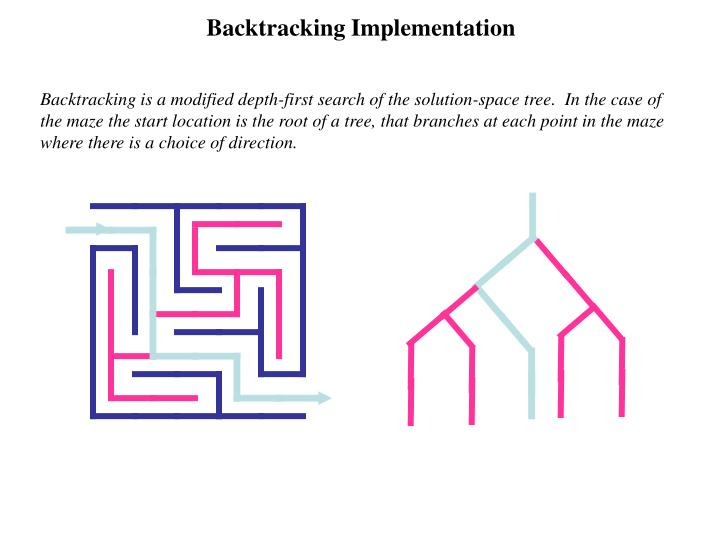
\includegraphics[width=0.80\textwidth, height=0.90\textheight]{figures/ilustra_backtracking_01.jpg}
%\caption{Realizar buscas com regiões reduzidas -- promissoras (regiões factíveis de soluções)}
\end{center}
\end{figure}
\end{frame}

%%%%%%%%%%%%%%%%%%%%%%%%%%%%%%%%%%%%%%%%%%%%%%%%%%%%%%%%%%%%%%%%%%%%%%%%%%%%%%%%%%%%%%%%%%

\begin{frame}[allowframebreaks=0.7]
\frametitle{\textit{Backtracking}}

Basicamente o procedimento do \textit{Backtracking} é definido por:

\begin{enumerate}

\item Inicia-se por  um casamento de um predicado \textit{backtrackable} $p$ com um outro predicado $p$.

\item Segue-se a execução da regra $p$, executando a instância das variáveis da \underline{esquerda para direita}.
 \textbf{Exemplo} (ilustrativo):\\
      \texttt{p(X1,X2,X3, ....., Xn) ?=> q1(X1), q2(X2), ...., qn(Xn).} 

\item Caso ocorra uma falha durante a execução da regra $p$,
 o compilador busca re-instanciar as variáveis do corpo de $p$ que falharem. Esta tentativa segue uma ordem:\\ 
  $q1(X1) \rightarrow q2(X2)\rightarrow ....\rightarrow qn(Xn)$, até a variável $Xn$

\item Caso $Xn$ seja instanciada com sucesso, tem-se uma resposta consistente para $p$

\item No caso de uma falha completa na regra corrente $p$, segue-se para uma próxima regra $p$
 (\texttt{p ....?=> ...}), a qual  é avaliada com novas instâncias as suas  variáveis.

\item Este processo é completo (exaustivo) e se repete até não for mais possível a reinstanciação de variáveis, ou ocorrer uma falha  durante a   execução.
\end{enumerate}
\end{frame}

%%%%%%%%%%%%%%%%%%%%%%%%%%%%%%%%%%%%%%%%%%%%%%%%%%%%%%%%%%%%%%%%%%%%%%%%%%%%%%%%%%%%%%%%%%

\begin{frame}[fragile]
\frametitle{Ilustra o \textit{Backtracking} -- Árvore de Busca}

\begin{figure}[!htb]
\begin{center}
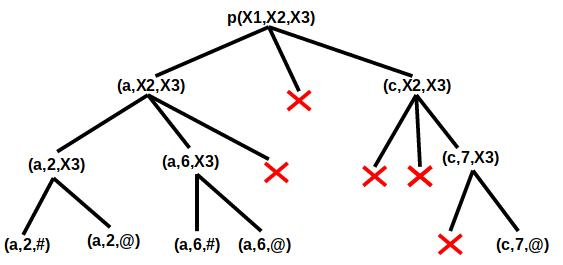
\includegraphics[width=0.950\textwidth, height=0.8\textheight]{figures/ilustra_backtracking_03.jpg}
%\caption{Realizar buscas com regiões reduzidas -- promissoras (regiões factíveis de soluções)}
\end{center}
\end{figure}
\textcolor{red}{Exercício: descubra os domínios possíveis de \texttt{X1}, \texttt{X2} e \texttt{X3}}
\end{frame}

%%%%%%%%%%%%%%%%%%%%%%%%%%%%%%%%%%%%%%%%%%%%%%%%%%%%%%%%%%%%%%%%%%%%%%%%%%%%%%%%%%%%%%%%%%

\begin{frame}[fragile]
\frametitle{Ilustra a Operacionalidade do \textit{Backtracking}}

\begin{figure}[!htb]
\begin{center}
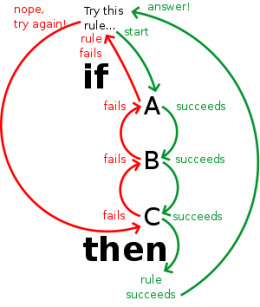
\includegraphics[width=0.60\textwidth, height=0.75\textheight]{figures/ilustra_backtracking_02.jpg}

\end{center}
\end{figure}

\end{frame}

%%%%%%%%%%%%%%%%%%%%%%%%%%%%%%%%%%%%%%%%%%%%%%%%%%%%%%%%%%%%%%%%%%%%%%%%%%%%%%%%%%%%%%%%%%

\begin{frame}[fragile]

\frametitle{Exemplo 01 -- Árvore Geneológica -- I}
 
Código:  \url{.../picat/uso_ancestral_recursao.pi}
\begin{lstlisting}[frame=single]
index (-,-) (+,-) (-,+)
ancestral(ana,maria).
ancestral(pedro,maria).
ancestral(maria,paula).
ancestral(paula,lucas).
ancestral(lucas, eduarda).

index (-)
mulher(ana).
mulher(maria).
mulher(paula).
mulher(eduarda).
homem(pedro).
homem(lucas).

....................................................continua
\end{lstlisting}
    
\end{frame}
\begin{frame}[fragile]

\frametitle{Exemplo 01 -- Árvore Geneológica -- II}
 
\begin{lstlisting}[frame=single]
....................................................
mae(X,Y) => ancestral(X,Y), mulher(X).
pai(X,Y) => ancestral(X,Y), homem(X).
avos(X,Y) => ancestral(X,Z), ancestral(Z,Y).

descende_de(X,Y) ?=> ancestral(Y,X).
descende_de(X,Y) => ancestral(Y,Z), descende_de(X,Z).

main ?=>
      descende_de(X,Y),
      prinitf("\n => %w descende de %w" , X,Y),
      false. 
main =>  true.
\end{lstlisting}
    
\end{frame}


%%%%%%%%%%%%%%%%%%%%%%%%%%%%%%%%%%%%%%%%%%%%%%%%%%%%%%%%%%%%%%%%%%%%%%%%%%%%%%%%%%%%%%%%%%

\begin{frame}[fragile]
\frametitle{Refletindo sobre o Exemplo}
    
    \begin{itemize}
        \item Uma chamada do tipo $mae(maria, X)$, seria como perguntar ao compilador
        ``\textit{Maria é mãe de quem ?}".
        
        \item Nesse caso o compilador  testa  possíveis valores que pudessem ser 
        unificados com $X$ satisfazendo a regra $mae(maria,X)$.
        
        \item Ou seja, seria como se estivéssemos perguntando:
        
        \begin{itemize}
            \item "Maria é mãe de Ana ?".
            \item "Maria é mãe de Paula ?".
            \item "Maria é mãe de Pedro ?".
        \end{itemize}
   \end{itemize}
    
\end{frame}


\begin{frame}[fragile]
\frametitle{Exemplo 02 -- Números -- I}

Código: \url{.../picat/backtracking_ex_02.pi}
\begin{scriptsize}

\begin{verbatim}
% $ picat backtracking_ex_02.pi 
% cl('backtracking_ex_02').
%%% FATOS ... 
index(-)  % fatos instanciados como retorno
    p(1).  p(3).   p(5).
	
index(-)  % fatos instanciados como retorno
    q(7).  q(4).  q(13).
	
%%%%%%%%%%%%%%%%%%%%%%%%%%%%%%%%%%%%%%%%%% 
algum_num(X, Y, Z) ?=> % ? esta regra tem backtracking
      p(X),
      q(Y),
      Z = 3,
      ((X + Y) mod Z) == 0.

algum_num(X, Y, Z) ?=>  % ? esta regra tem backtracking
      p(X),
      q(Y),
      Z = 4,
      ((X + Y) mod Z) == 0.
............................................ continua
 \end{verbatim} 

\end{scriptsize}
\end{frame}


\begin{frame}[fragile]
\frametitle{Exemplo 02 -- Números -- II}

\begin{scriptsize}
\begin{verbatim}
........................................
algum_num(X, Y, Z) =>  % esta regra NAO tem backtracking
      p(X),
      q(Y),
      Z = 5,
      ((X + Y) mod Z) == 0.

% CUIDAR AQUI
%algum_num(_, _, _)  =>     
%     printf("\n NAO HA MAIS MULTIPLOS de 3, 4 ou 5").    
%%%%%%%%%%%%%%%%%%%%%%%%%n%%%%%%%%%%%%%%%%% %%%%%%%%%%%%%%%
main ?=>  % main com backtracking
   algum_num( X, Y, Z),
   imp(X,Y,Z),
   false.     % força TODAS respostas 
   
main => imp_tracejados(40).   
 \end{verbatim} 
 
 \end{scriptsize}
\end{frame}

\begin{frame}[fragile]
\frametitle{Exemplo 02 -- Saída}

\begin{scriptsize}
\begin{verbatim}
$ picat backtracking_ex_02.pi 

 X:5  Y:7 	X+Y:12 é MULTIPLO de:3
 X:5  Y:4 	X+Y:9 é MULTIPLO de:3
 X:5  Y:13 	X+Y:18 é MULTIPLO de:3
 X:1  Y:7 	X+Y:8 é MULTIPLO de:4
 X:3  Y:13 	X+Y:16 é MULTIPLO de:4
 X:5  Y:7 	X+Y:12 é MULTIPLO de:4
 X:1  Y:4 	X+Y:5 é MULTIPLO de:5
 X:3  Y:7 	X+Y:10 é MULTIPLO de:5
========================================
$ 
\end{verbatim} 
  \end{scriptsize}   
  
\textcolor{red}{Cuidar em confundir \textbf{0} (zero) com \textbf{O}. Perdi horas no código acima.}  
\end{frame}








\begin{frame}[fragile]
\frametitle{Reflexões}


\begin{itemize}
\item A recursão é o paradigma das linguagens declarativas como Haskell, Prolog, Picat, ... etc
 
 \pause
 \item As regras recursivas são construídas com uma ou mais  \textcolor{magenta}{\textit{regras aterradas}}, que  \textcolor{magenta}{\textbf{sempre vem antes}} das demais
 regras recursivas, as  quais podem ou não terem o \textit{backtracking} habilitados ( \textcolor{magenta}{\textbf{\texttt{?=>}}})
 
 
 \pause
 \item A avaliação destas regras \textcolor{magenta}{\textbf{são sempre da esquerda para direita}}, ocorrendo o \textcolor{magenta}{\textit{backtracking}} em caso de falha ou de uma nova resposta
  
  \pause
 \item As regras recursivas com \textit{backtracking} habilitados ( \textbf{\texttt{?=>}} ), apenas
 para regras predicativas.  \textcolor{red}{As funções não admitem \textit{backtracking}!}
 
  \pause
 \item \textcolor{green}{A metodologia destas regras e sua construção, seguem  esquemas mais
 avançados da programação declarativa!}
 
%  \pause
% \item O \textbf{\textit{main}} é uma regra predicativa que pode conter ou não argumentos.
 
 
\end{itemize}

\end{frame}
%%%%%%%%%%%%%%%%%%%%%%%%%%%%%%%%%%%%%%%%%%%%%%%%%%%%%%%%%%%%%%%%%%%%%%%%%%%%%%%%%%%%%%%%%%
